% Options for packages loaded elsewhere
\PassOptionsToPackage{unicode}{hyperref}
\PassOptionsToPackage{hyphens}{url}
%
\documentclass[
  12pt,
  a4paper,
]{scrartcl}
\usepackage{amsmath,amssymb}
\usepackage{setspace}
\usepackage{iftex}
\ifPDFTeX
  \usepackage[T1]{fontenc}
  \usepackage[utf8]{inputenc}
  \usepackage{textcomp} % provide euro and other symbols
\else % if luatex or xetex
  \usepackage{unicode-math} % this also loads fontspec
  \defaultfontfeatures{Scale=MatchLowercase}
  \defaultfontfeatures[\rmfamily]{Ligatures=TeX,Scale=1}
\fi
\usepackage{lmodern}
\ifPDFTeX\else
  % xetex/luatex font selection
\fi
% Use upquote if available, for straight quotes in verbatim environments
\IfFileExists{upquote.sty}{\usepackage{upquote}}{}
\IfFileExists{microtype.sty}{% use microtype if available
  \usepackage[]{microtype}
  \UseMicrotypeSet[protrusion]{basicmath} % disable protrusion for tt fonts
}{}
\usepackage{xcolor}
\usepackage[left=3cm,right=2cm,top=3cm,bottom=2cm]{geometry}
\usepackage{longtable,booktabs,array}
\usepackage{calc} % for calculating minipage widths
% Correct order of tables after \paragraph or \subparagraph
\usepackage{etoolbox}
\makeatletter
\patchcmd\longtable{\par}{\if@noskipsec\mbox{}\fi\par}{}{}
\makeatother
% Allow footnotes in longtable head/foot
\IfFileExists{footnotehyper.sty}{\usepackage{footnotehyper}}{\usepackage{footnote}}
\makesavenoteenv{longtable}
\usepackage{graphicx}
\makeatletter
\def\maxwidth{\ifdim\Gin@nat@width>\linewidth\linewidth\else\Gin@nat@width\fi}
\def\maxheight{\ifdim\Gin@nat@height>\textheight\textheight\else\Gin@nat@height\fi}
\makeatother
% Scale images if necessary, so that they will not overflow the page
% margins by default, and it is still possible to overwrite the defaults
% using explicit options in \includegraphics[width, height, ...]{}
\setkeys{Gin}{width=\maxwidth,height=\maxheight,keepaspectratio}
% Set default figure placement to htbp
\makeatletter
\def\fps@figure{htbp}
\makeatother
\setlength{\emergencystretch}{3em} % prevent overfull lines
\providecommand{\tightlist}{%
  \setlength{\itemsep}{0pt}\setlength{\parskip}{0pt}}
\setcounter{secnumdepth}{-\maxdimen} % remove section numbering
\newlength{\cslhangindent}
\setlength{\cslhangindent}{1.5em}
\newlength{\csllabelwidth}
\setlength{\csllabelwidth}{3em}
\newlength{\cslentryspacingunit} % times entry-spacing
\setlength{\cslentryspacingunit}{\parskip}
\newenvironment{CSLReferences}[2] % #1 hanging-ident, #2 entry spacing
 {% don't indent paragraphs
  \setlength{\parindent}{0pt}
  % turn on hanging indent if param 1 is 1
  \ifodd #1
  \let\oldpar\par
  \def\par{\hangindent=\cslhangindent\oldpar}
  \fi
  % set entry spacing
  \setlength{\parskip}{#2\cslentryspacingunit}
 }%
 {}
\usepackage{calc}
\newcommand{\CSLBlock}[1]{#1\hfill\break}
\newcommand{\CSLLeftMargin}[1]{\parbox[t]{\csllabelwidth}{#1}}
\newcommand{\CSLRightInline}[1]{\parbox[t]{\linewidth - \csllabelwidth}{#1}\break}
\newcommand{\CSLIndent}[1]{\hspace{\cslhangindent}#1}
\ifLuaTeX
\usepackage[bidi=basic]{babel}
\else
\usepackage[bidi=default]{babel}
\fi
\babelprovide[main,import]{brazilian}
% get rid of language-specific shorthands (see #6817):
\let\LanguageShortHands\languageshorthands
\def\languageshorthands#1{}
\ifLuaTeX
  \usepackage{selnolig}  % disable illegal ligatures
\fi
\IfFileExists{bookmark.sty}{\usepackage{bookmark}}{\usepackage{hyperref}}
\IfFileExists{xurl.sty}{\usepackage{xurl}}{} % add URL line breaks if available
\urlstyle{same}
\hypersetup{
  pdftitle={Título do Artigo},
  pdfauthor={Nome Sobrenome¹; Outro Nome²},
  pdflang={pt-BR},
  pdfkeywords={palavra-chave 1, palavra-chave 2, palavra-chave 3},
  hidelinks,
  pdfcreator={LaTeX via pandoc}}

\title{Título do Artigo}
\usepackage{etoolbox}
\makeatletter
\providecommand{\subtitle}[1]{% add subtitle to \maketitle
  \apptocmd{\@title}{\par {\large #1 \par}}{}{}
}
\makeatother
\subtitle{Subtítulo (opcional)}
\author{Nome Sobrenome¹ \and Outro Nome²}
\date{21 setembro 2025}

\begin{document}
\maketitle

\renewcommand*\contentsname{Sumário}
{
\setcounter{tocdepth}{2}
\tableofcontents
}
\setstretch{1.5}
\hypertarget{resumo}{%
\subsection{Resumo}\label{resumo}}

Escreva aqui um \textbf{resumo} conciso (150--250 palavras) apresentando
o tema, objetivo(s), método(s), resultado(s) principais e
conclusão(ões). O resumo deve ser \textbf{informativo} e
autossuficiente, sem citações extensas nem abreviações não definidas.

\textbf{Palavras-chave:} palavra-chave 1; palavra-chave 2; palavra-chave
3.

\hypertarget{abstract-opcional}{%
\subsubsection{Abstract (opcional)}\label{abstract-opcional}}

Short version of the abstract in English (if required by the venue).\\
\textbf{Keywords:} keyword 1; keyword 2; keyword 3.

\hypertarget{introduuxe7uxe3o}{%
\section{Introdução}\label{introduuxe7uxe3o}}

Contextualize o problema, a motivação e os objetivos do estudo.
Apresente brevemente a lacuna na literatura e contribuições do artigo.
Cite trabalhos relevantes no fluxo do texto, por exemplo, segundo Silva
(\protect\hyperlink{ref-silva2020}{2020}), a estruturação do projeto
influencia a qualidade dos resultados; estudos recentes reforçam esse
ponto (\protect\hyperlink{ref-souza2022}{Souza; Pereira, 2022}).

\hypertarget{referencial-teuxf3rico-ou-revisuxe3o-de-literatura}{%
\section{Referencial teórico (ou Revisão de
literatura)}\label{referencial-teuxf3rico-ou-revisuxe3o-de-literatura}}

Organize os conceitos, definições e trabalhos relacionados. Use citações
\textbf{narrativas} (ex.: \emph{Silva (2020) discute\ldots{}}) ou
\textbf{parentéticas} (ex.: \emph{\ldots{} já observado (SILVA, 2020)}),
conforme o estilo ABNT aplicado automaticamente pelo CSL.

\hypertarget{metodologia}{%
\section{Metodologia}\label{metodologia}}

Descreva o delineamento do estudo, materiais e métodos, escopo,
critérios de inclusão/exclusão, instrumentos, procedimentos e forma de
análise dos dados. Detalhe o suficiente para permitir
\textbf{reprodutibilidade}.

\hypertarget{resultados}{%
\section{Resultados}\label{resultados}}

Apresente os resultados de forma clara, com \textbf{tabelas} e
\textbf{figuras} quando necessário.

\begin{longtable}[]{@{}lll@{}}
\caption{Tabela 1 -- Desempenho comparativo}\tabularnewline
\toprule\noalign{}
Métrica & Grupo A & Grupo B \\
\midrule\noalign{}
\endfirsthead
\toprule\noalign{}
Métrica & Grupo A & Grupo B \\
\midrule\noalign{}
\endhead
\bottomrule\noalign{}
\endlastfoot
Acurácia (\%) & 92,3 & 88,7 \\
Tempo (s) & 12,4 & 10,9 \\
\end{longtable}

\emph{Fonte: elaboração própria.}

\begin{figure}
\centering
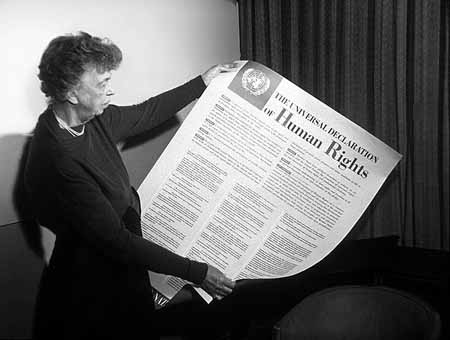
\includegraphics{images/Eleanor_Roosevelt_and_Human_Rights_Declaration.jpeg}
\caption{Exemplo de figura com legenda.}
\end{figure}

\emph{Figura 1 -- Fluxo resumido do método. Fonte: elaboração própria.}

\hypertarget{discussuxe3o}{%
\section{Discussão}\label{discussuxe3o}}

Interprete os achados à luz da literatura, a plausibilidade dos
resultados, limitações do estudo e implicações práticas/teóricas.
Compare com trabalhos anteriores (e.g., ver Souza; Pereira
(\protect\hyperlink{ref-souza2022}{2022})).

\hypertarget{conclusuxe3o}{%
\section{Conclusão}\label{conclusuxe3o}}

Resuma as respostas aos objetivos, destaque contribuições e trabalhos
futuros. Evite intro

\hypertarget{bibliography}{%
\section*{Referências}\label{bibliography}}
\addcontentsline{toc}{section}{Referências}

\hypertarget{refs}{}
\begin{CSLReferences}{0}{1}
\leavevmode\vadjust pre{\hypertarget{ref-silva2020}{}}%
SILVA, João P. \textbf{Introdução à Pesquisa Científica}. São Paulo:
Editora Acadêmica, 2020.

\leavevmode\vadjust pre{\hypertarget{ref-souza2022}{}}%
SOUZA, Maria A.; PEREIRA, Carlos H.
\href{https://doi.org/10.1234/rbpo.v42i3.2022}{Modelagem e otimização em
sistemas discretos}. \textbf{Revista Brasileira de Pesquisa
Operacional}, {[}\emph{s. l.}{]}, v. 42, n. 3, p. 123--145, 2022.

\end{CSLReferences}

\end{document}
